\documentclass[10pt,landscape,a4paper]{article}
\usepackage[utf8]{inputenc}
\usepackage[ngerman]{babel}
\usepackage[T1]{fontenc}
%\usepackage[LY1,T1]{fontenc}
%\usepackage{frutigernext}
%\usepackage[lf,minionint]{MinionPro}
\usepackage{tikz}
\usetikzlibrary{shapes,positioning,arrows,fit,calc,graphs,graphs.standard}
\usepackage[nosf]{kpfonts}
\usepackage[t1]{sourcesanspro}
\usepackage{multicol}
\usepackage{wrapfig}
\usepackage[top=0mm,bottom=1mm,left=0mm,right=1mm]{geometry}
\usepackage[framemethod=tikz]{mdframed}
\usepackage{microtype}
\usepackage{pdfpages}
\usepackage[linguistics]{forest}

\let\bar\overline

\definecolor{myblue}{cmyk}{1,.72,0,.38}

\def\firstcircle{(0,0) circle (1.5cm)}
\def\secondcircle{(0:2cm) circle (1.5cm)}

\colorlet{circle edge}{myblue}
\colorlet{circle area}{myblue!5}

\tikzset{filled/.style={fill=circle area, draw=circle edge, thick},
    outline/.style={draw=circle edge, thick}}
    
\pgfdeclarelayer{background}
\pgfsetlayers{background,main}

\everymath\expandafter{\the\everymath \color{myblue}}
\everydisplay\expandafter{\the\everydisplay \color{myblue}}

\renewcommand{\baselinestretch}{.8}
\pagestyle{empty}

\global\mdfdefinestyle{header}{%
linecolor=gray,linewidth=1pt,%
leftmargin=0mm,rightmargin=0mm,skipbelow=0mm,skipabove=0mm,
}

\newcommand{\header}{
\begin{mdframed}[style=header]
\scriptsize
\sffamily
Hilfszettel zur Klausur\\
von~Tim~S.,~Seite~\thepage~von~2
\end{mdframed}
}

\makeatletter % Author: https://tex.stackexchange.com/questions/218587/how-to-set-one-header-for-each-page-using-multicols
\renewcommand{\section}{\@startsection{section}{1}{0mm}%
                                {.2ex}%
                                {.2ex}%x
                                {\color{myblue}\sffamily\small\bfseries}}
\renewcommand{\subsection}{\@startsection{subsection}{1}{0mm}%
                                {.2ex}%
                                {.2ex}%x
                                {\sffamily\bfseries}}



\def\multi@column@out{%
   \ifnum\outputpenalty <-\@M
   \speci@ls \else
   \ifvoid\colbreak@box\else
     \mult@info\@ne{Re-adding forced
               break(s) for splitting}%
     \setbox\@cclv\vbox{%
        \unvbox\colbreak@box
        \penalty-\@Mv\unvbox\@cclv}%
   \fi
   \splittopskip\topskip
   \splitmaxdepth\maxdepth
   \dimen@\@colroom
   \divide\skip\footins\col@number
   \ifvoid\footins \else
      \leave@mult@footins
   \fi
   \let\ifshr@kingsaved\ifshr@king
   \ifvbox \@kludgeins
     \advance \dimen@ -\ht\@kludgeins
     \ifdim \wd\@kludgeins>\z@
        \shr@nkingtrue
     \fi
   \fi
   \process@cols\mult@gfirstbox{%
%%%%% START CHANGE
\ifnum\count@=\numexpr\mult@rightbox+2\relax
          \setbox\count@\vsplit\@cclv to \dimexpr \dimen@-1cm\relax
\setbox\count@\vbox to \dimen@{\vbox to 1cm{\header}\unvbox\count@\vss}%
\else
      \setbox\count@\vsplit\@cclv to \dimen@
\fi
%%%%% END CHANGE
            \set@keptmarks
            \setbox\count@
                 \vbox to\dimen@
                  {\unvbox\count@
                   \remove@discardable@items
                   \ifshr@nking\vfill\fi}%
           }%
   \setbox\mult@rightbox
       \vsplit\@cclv to\dimen@
   \set@keptmarks
   \setbox\mult@rightbox\vbox to\dimen@
          {\unvbox\mult@rightbox
           \remove@discardable@items
           \ifshr@nking\vfill\fi}%
   \let\ifshr@king\ifshr@kingsaved
   \ifvoid\@cclv \else
       \unvbox\@cclv
       \ifnum\outputpenalty=\@M
       \else
          \penalty\outputpenalty
       \fi
       \ifvoid\footins\else
         \PackageWarning{multicol}%
          {I moved some lines to
           the next page.\MessageBreak
           Footnotes on page
           \thepage\space might be wrong}%
       \fi
       \ifnum \c@tracingmulticols>\thr@@
                    \hrule\allowbreak \fi
   \fi
   \ifx\@empty\kept@firstmark
      \let\firstmark\kept@topmark
      \let\botmark\kept@topmark
   \else
      \let\firstmark\kept@firstmark
      \let\botmark\kept@botmark
   \fi
   \let\topmark\kept@topmark
   \mult@info\tw@
        {Use kept top mark:\MessageBreak
          \meaning\kept@topmark
         \MessageBreak
         Use kept first mark:\MessageBreak
          \meaning\kept@firstmark
        \MessageBreak
         Use kept bot mark:\MessageBreak
          \meaning\kept@botmark
        \MessageBreak
         Produce first mark:\MessageBreak
          \meaning\firstmark
        \MessageBreak
        Produce bot mark:\MessageBreak
          \meaning\botmark
         \@gobbletwo}%
   \setbox\@cclv\vbox{\unvbox\partial@page
                      \page@sofar}%
   \@makecol\@outputpage
     \global\let\kept@topmark\botmark
     \global\let\kept@firstmark\@empty
     \global\let\kept@botmark\@empty
     \mult@info\tw@
        {(Re)Init top mark:\MessageBreak
         \meaning\kept@topmark
         \@gobbletwo}%
   \global\@colroom\@colht
   \global \@mparbottom \z@
   \process@deferreds
   \@whilesw\if@fcolmade\fi{\@outputpage
      \global\@colroom\@colht
      \process@deferreds}%
   \mult@info\@ne
     {Colroom:\MessageBreak
      \the\@colht\space
              after float space removed
              = \the\@colroom \@gobble}%
    \set@mult@vsize \global
  \fi}

\makeatother
\setlength{\parindent}{0pt}

\begin{document}
\graphicspath{ {inhalt/pictures/} }
%\footnotesize
\small
\begin{multicols*}{6}
\section{Recap}
\scriptsize{Abstract Data Type (ADT)} {\tiny an object with well-defined operations, e.g. a stack supports push() and pop() operations \\
can be implemented using different data structures, e.g. a stack can be implemented using a linked list or an array}\\
\scriptsize{Array} {\tiny a contiguous sequence of
objects with the same size \\
close to how computers store data in their memory\\
can also be multi-dimensional\\
support fast access to their elements through indexing\\
resizing and inserting values in arbitrary locations are expensive\\
in python: no built-in data structure, lists are indexable, use numpy library for proper/faster arrays
}\\
\scriptsize{Lists}
{\tiny main operations: append/prepend, head/tail\\
typically implemented usingn linked lists (python lists are array-based)
}\\
\scriptsize{Stacks} {\tiny last-in-first-out (LIFO) data structure\\
basic operations: push, pop\\
can be implemented using linked lists (or arrays)
}\\
\scriptsize{Queues} {\tiny first-in-first-out (FIFO) data structure\\
basic operations: enqueue, dequeue\\
can be implemented using linked lists (or maybe arrays)
}\\
\scriptsize{Strings} {\tiny often implemented based on character arrays }\\
\scriptsize{Maps/Dictionaries} {\tiny similar to arrays and lists, but allow indexing with (almost) arbitrary data types\\
maps generally implemented using hashing }\\
\scriptsize{Sets} {\tiny implement the mathematical (finite) sets, a collection of unique elements without order}\\
\scriptsize{Algorithms}
{\tiny Desirable properties: correctness, robustness, efficiency, simplicity}\\
\scriptsize{Resursion}
{\tiny have to define one or more base cases\\
each recursive step should approach the base case}
\section{Analysis of Algorithms}
{\tiny characterize running times of algorithms as a function of input size:\\
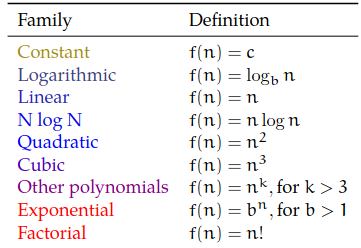
\includegraphics[scale=0.25]{functions.png}
}\\
\scriptsize{Logarithm} {\tiny the inverse of exponentiation: x = logb n -> b**x = n \\
for us, no base means base-2 \\
log xy = log x + log y \\
log (x/y) = log x - log y \\
log x**a = a log x \\
logb x = logk x / logk b\\
grow much slower than linear functions
}\\
\scriptsize{Polynomials} {\tiny degree-0: f(n) = c\\
degree-1: f(n)=n+c\\
degree-2: f(n)=n**2+n+c\\
generally drop the lower order terms\\
1+2+3+...+n = n(n+1)/2
}\\
\scriptsize{Permutations}\\ 
{\tiny n! = n*(n-1)*...*2*1\\
P(n,k) = n*(n-1)*...*(n-k-1) = n!/(n-k)!} \\
\scriptsize{Combinations}\\ 
{\tiny n choose k C(n,k) = P(n.k)/P(k,k) = n!/(n-k)!*k!\\
P(n,k) = n*(n-1)*...*(n-k-1) = n!/(n-k)!}\\
\scriptsize{Proof by induction}\\ 
{\tiny used for both proving the correctness and running times of algorithms\\
show that the base case holds\\
assume the result is correct for n, show that it also holds for n+1
}\\
\scriptsize{Hardware independence} {\tiny characterized by random access memory (RAM)\\
the data and instructions are stored in the RAM\\
processing unit performs basic operations in constant time\\
any memory cell with an address can be accessed in equal (constant) time\\
the processor fetches them as needed and executes following the instruction\\
there may be other, specialized registers\\
modern processing units also employ a cache
}\\
\scriptsize{Formal analysis of running time} {\tiny simply count the number of primitive operations\\
primitive operations include: assignment, arithmetic operations, compare primitive data types (in Java: boolean, byte, char, short, int, long, float and double), access a single memory location, function calls, return from functions\\
non-primitive operations: loops, recursion, compare sequences
}\\
\scriptsize{Big-O notation} {\tiny used for indicating an upper bound of an algorithm as a function of running time\\
if running time of an algorithm is O(f(n)), its running time grows proportional to f(n) as the input size n grows\\
drop the constants and lower order terms\\
transitivity: if f(n)=O(g(n)), and g(n)=O(h(n)), then f(n)=O(h(n))\\
additivity: if both f(n) and g(n) are O(h(n)), f(n)+g(n)=O(h(n))
}\\
\scriptsize{maximum problem size} {\tiny 
asymptotic analysis is important: assume we can solve a problem of size m in a given time on current hardware, when we get a better computer, we can calculate the new problem size we can solve in the same time\\
gap between polynomial and exponential algorithms: problem size for exponential algorithms does not scale with faster computers
}\\
\scriptsize{worst case analysis}\\ {\tiny in most cases we are interested in the worst case analysis \\
average case analysis is also useful, but requires defining a distribution over possible inputs and is often more challenging\\
pro: easier, get a very strong guarantee that the algorithm won't perform worse than the bound\\
con: in some problems, worst case examples are very rare
}\\
\scriptsize{asymptotic analysis}\\ {\tiny our analyses are based on asymptotic behavior \\
pro: correct for a 'large enough' input\\
con: constant or lower order factors are not always unimportant
}\\
\scriptsize{Big-O relatives} {\tiny Big-O(upper bound): f(n) is O(g(n)) if f(n) is asymptotically less than or equal to g(n)\\
Big-Omega (lower bound): f(n) is Omega(g(n)) if f(n) is asymptotically greater than or equal to g(n)\\
Big-Theta (upper/lower bound): f(n) is Theta(g(n)) if f(n) is asymptotically equal to g(n): f(n) is O(g(n)) and f(n) is Omega(g(n))
}\\
\scriptsize{Summary} {\tiny sublinear (e.g. logarithmic), linear, and nlogn algorithms are good\\
polynomial algorithms may be acceptable in many cases\\
exponential algorithms are bad
}
\section{Algorithmic patterns}
\scriptsize{Recursion}\\
{\tiny recursion depth:\\
compilers/interpreters allocate space on a stack for the bookkeeping for each function call\\
most environments limit the number of recursive calls: long chains of recursion are likely to cause errors
}\\
{\tiny tail recursion:\\
e.g. linear search \\
easy to convert to iteration\\
easy to optimize, and optimized by many compilers (not by the Python interpreter)
}\\
\scriptsize{Brute force}
{\tiny in some cases we may need to enumerate all possible cases (e.g. to find the best solution)\\
common in combinatorial problems\\
often intractable, practical only for small input sizes\\
the beginning of finding a more efficient approach\\
example: segmentation
}\\
\scriptsize{Divide and conquer}
{\tiny divide the problem into smaller parts until it becomes trivial to solve\\
once small parts are solved, results are combined\\
goes well with recursion\\
a particular flavor: binary search (sometimes called decrease and conquer)\\
example: nearest neighbors, merge sort, quick sort, integer multiplication, matrix multiplication, fast Furrier transform\\
not always yield good results, cost of merging should be less than the gain from the divisions
}\\
\scriptsize{Greedy algorithm} 
{\tiny optimizes a local constraint\\
results in correct solutions for some problems, in others they may result in "good enough" solutions\\
efficient if works\\
examples: graph algorithms (find shortest paths, scheduling)\\
e.g. produce minimum number of coins for a particular sum s (not correct for coins of 10, 30, 40 and sum value of 60)
}\\
\scriptsize{Dynamic programming} 
{\tiny save earlier results to reduce computation\\
sometimes called memoization\\
examples: common parsing algorithms, Fibonacci
}\\
\scriptsize{Others}
{\tiny backtracking, branch-and-bound;
randomized algorithms;
distributed algorithms (sometimes called swarm optimization);
transformation 
}
\section{Sorting}
\scriptsize{Bubble sort}\\ 
{\tiny compare first 2 elements, swap if not in order \\
shift and compare the next 2 elements, again swap if needed \\
when read the end, repeat the process from the beginning unless there were no swaps in the last iteration \\
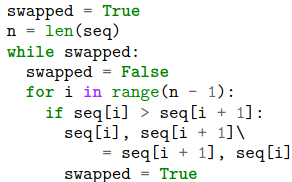
\includegraphics[scale=0.25]{bubble_sort.png}\\
concerns: many swaps, in-place\\
not practical, not used in practice
}\\
\scriptsize{Insertion sort}\\
{\tiny assume the elements arrive one by one, and we have a sorted sequence \\
shift all elements larger than the new one to the right\\
put the new element in its correct place\\
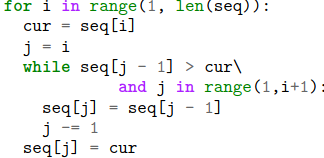
\includegraphics[scale=0.25]{insertion-sort.png}\\
performs reasonably fast for sorting short sequences, on longer sequences, performs worse than more advanced algorithms like merge sort or quick sort\\
in practice faster than bubble sort and selection sort\\
online: sort items as they arrive\\
stable: do not swap elements with equal keys\\
adaptive: faster if order of elements closer to sorted sequence
}\\
\scriptsize{Merge sort}\\
{\tiny split the sequence \\
sort the subsequences\\
merge the sorted lists\\
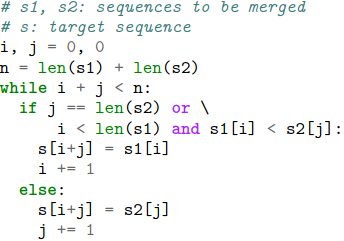
\includegraphics[scale=0.25]{merge-sort_1.png}\\
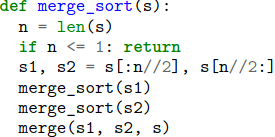
\includegraphics[scale=0.25]{merge-sort_2.png}\\
log n splits\\
particular useful for settings with low random-access memory, or sequential access\\
well-studied, many variants (in-place, non-recursive)
}\\
\scriptsize{Quicksort}\\
{\tiny another popular divide-and-conquer sorting algorithm \\
the big part of the work is done before splitting\\
worst time complexity is O(n**2), but in practice performs better than merge sort on average\\
pick a pivot p, and divide the sequence into 3 parts:\\
L: smaller than p\\
G: larger than p\\
E: equal to p\\
sort L and G recursively\\
combination is simple concatenation\\
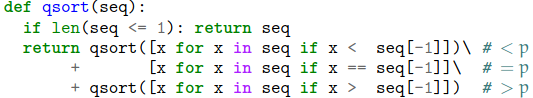
\includegraphics[scale=0.25]{quicksort.png}\\
similar to merge sort, performs O(n) operations at each level in recursion\\
overall complexity is proportional to n*depthOfTree\\
unlike merge sort, no balanced-tree guarantee, in the worst case the depth of the tree can be n, resulting in O(n**2) complexity\\
worst case: when input sequence is sorted\\
randomized quicksort: pick the pivot randomly\\
best case: pick the median of the sequence as pivot, but finding median requires O(nlogn)\\
common apprach: pick 3 values (typically first, middle, last) and select the median\\
can be easily implemented in-place\\
}\\
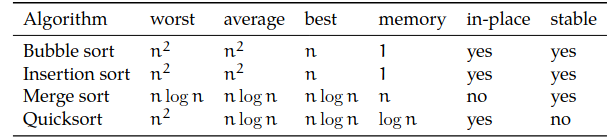
\includegraphics[scale=0.23]{sorting.png}\\
\scriptsize{Bucket sort}\\
{\tiny puts elements of the input into a pre-defined number of ordered 'buckets' \\
elements in each bucket is sorted (typically using insertion sort, worst case O(n**2)\\
can retrieve the sorted elements by visiting each bucket\\
does not compare elements to each other when deciding which bucket to place them\\
in speical cases results in O(n) worst-case complexity (as many buckets as keys)
}\\
\scriptsize{Radix sort}\\
{\tiny sort objects with multiple keys\\
define the order of key pairs as (k1,l1)<(k2,l2) if k1<k2, or k1=k2 and l1<l2, can be generalized to key tuples of any length\\
also known as lexicographic or dictionary order\\
use multiple stable bucket sorts for this purpose
} 
\section{Trees}
{\tiny a hierarchical, non-linear data structure \\
a graph with certain properties\\
in cl: parse trees, language trees, decision trees}\\
\scriptsize{Definitions}\\ {\tiny a set of nodes organized hierarchically with the following properties: \\
If a tree is non-empty, it has a special node root\\
Except the root node, every node in the tree has a unique parent (all nodes except the root are children of another node)\\
Alternatively, recursive definition:\\
the empty set of nodes is a tree\\
otherwise a tree contains a root with sub-trees as its children}\\
\scriptsize{siblings} {\tiny nodes with the same parent
}\\
\scriptsize{internal nodes} {\tiny nodes with children
}\\
\scriptsize{leaf nodes} {\tiny nodes without children
}\\
\scriptsize{path} {\tiny sequence of connected nodes
}\\
\scriptsize{ancestors/decendants} {\tiny any node in the path from the root to a particular node; a node is the descendant of its ancestors
}\\
\scriptsize{internal nodes} {\tiny nodes with children
}\\
\scriptsize{subtree} {\tiny a tree rooted by a non-root node
}\\
\scriptsize{depth} {\tiny number of edges from root
}\\
\scriptsize{height} {\tiny number of edges from the deepest descendant; the height of a tree is the height of its root
}\\
\scriptsize{Ordered trees}\\ 
{\tiny if there is an odering between siblings, e.g. document (e.g. HTML) structure tree, parse trees, family tree\\
in many cases order is not important (e.g. class hierarchy in object-oriented program, file tree in computer)
}\\
\scriptsize{Binary trees}\\
{\tiny nodes can have at most 2 children\\
have a natural order: left/right child\\
proper/full: if every node has either 2 children or none\\
complete: if every level except possibly the last is completely filled, all nodes at the last level is at the left\\
perfect: a full binary tree whose leaf nodes have the same depth\\
properties: for a binary tree with nl leaf nodes, ni internal nodes, n nodes and height h:\\
h+1 <= n <= 2**(h+1)-1\\
1 <= nl <= 2**h\\
h <= ni <= 2**h -1\\
log(n+1)-1 <= h <= n-1\\
for any proper binary tree: nl=ni+1
}\\
\scriptsize{Implementation} \\
{\tiny general case: linked data structure\\
arrays: root stored at index 0, left child of the node at index i stored at 2i+1, right child at 2i+2, parent at (i-1)/2 (if the binary tree is complete, this representation does not waste (much) space
}\\
\scriptsize{Breadth first traversal (level order)}\\ 
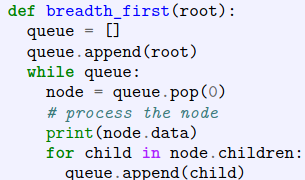
\includegraphics[scale=0.25]{breath_first.png}\\
\scriptsize{Pre-order traversal} \\
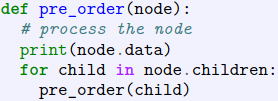
\includegraphics[scale=0.25]{pre-order.png}\\
\scriptsize{Post-order traversal} \\
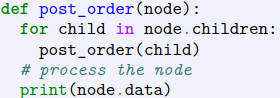
\includegraphics[scale=0.25]{post-order.png}\\
\scriptsize{In-order traversal} \\
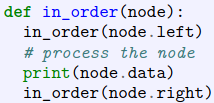
\includegraphics[scale=0.25]{in-order.png}
\section{Priority Queues}
{\tiny a collection, an abstract data type, that stores items (key-value pairs)\\
key: priority of the item\\
value: actual data of interest\\
its interface similar to a standard queue, but the item with the highest priority (minimum or maximum key value) instead of the first item entered into the queue is removed\\
applications ranging from data compression to discrete optimization
}\\
\scriptsize{Operations}\\ {\tiny insert(k,v): similar to enqueue(v)\\
remove(): similar to dequeue(), often called remove-min() or remove-max() depending on minimum or maximum key value that is considered having the highest priority
}\\
\scriptsize{Implementation}\\ 
{\tiny unsorted list: insert O(1), remove O(n)\\
sorted list: insert O(n), remove O(1)\\
binary heap: insert O(logn), remove O(logn)\\
(some improvements:\\
d-ary heaps: insert O(logd n), remove O(dlogd n)\\
fibonacci heaps: insert O(1), remove O(logn)
}\\
\scriptsize{Sorting with priority queues}\\ 
{\tiny implemented with sorted list: = insertion sort O(n**2)\\
use unsorted list: = selection sort O(n**2)\\
use binary heap: = heap sort O(nlogn) (not stable; not in-place: needs O(n) extra space\\
in-place heap sort:\\
1. bottom-up heap construction\\
2. iteratively remove the maximum element and place it at the end\\
efficiency: heap construction O(n) + n*remove-min O(nlogn) = O(nlogn)
}

\section{Binary Heaps}
{\tiny a binary tree where the nodes store items with an ordering relation 
}\\
\scriptsize{Properties}\\ 
{\tiny shape: a complete binary tree (all levels of the tree, except possibly the last one, are full; all empty slots (if any) are to the right of the filled nodes at the lowest level)\\
heap order: max-heap: parents' keys larger than children's keys; min-heap: parents' keys smaller than children's keys
}\\
\scriptsize{Height} {\tiny log n\\
at least 2**h nodes -> h<=logn\\
at most 2**(h+1)-1 nodes -> h>=log(n+1)-1
}\\
\scriptsize{add new item}\\
{\tiny add to the first available slot\\
bubble up until the heap property is satisfied\\
at most h=logn comparisons/swaps
}\\
\scriptsize{remove the min/max}\\ 
{\tiny item to be removed is at the root\\
replace root with the element at the last slot\\
bubble down until the heap property is satisfied
}\\
\scriptsize{implementation} {\tiny can be stored efficiently using an array data structure (like any complete binary tree)
}\\
\scriptsize{construction} {\tiny for n items, we can construct a heap by inserting each key in O(nlogn) time\\
Bottom-up construction (O(n) complexity) (if we have the complete list):\\
1. fill the leaf nodes (h=logn, num of internal nodes=2**h-1, num of leaf nodes=n-2**h-1\\
2. fill the next level, bubble down if necessary\\
3. repeat 2 until all elements are inserted and heap property is satisfied
}\\
\scriptsize{Python standard heap implementation} {\tiny heapq module\\
allows maintaining a list(array) based heap\\
heappush(h,e): insert e(a key-value tuple) into heap h\\
heappop(h): return the minimum value from heap h\\
heapify(h): construct a heap from given list heappos(h)
}

\section{Graphs}
{\tiny collection of vertices(nodes) connected pairwise by edges(arcs) \\
edges can be directed (also called arcs, 2-tuples or ordered pairs) and undirected (unordered pairs, or pair sets)
}\\
\scriptsize{applications}\\ 
{\tiny city maps, chemical formulas, neural networks, ANNs, electronic circuits, computer networks, infectious diseases, probability distributions, word semantics\\
food web, course dependencies, social media, scheduling, games, academic networks, inheritance relations in OOP, flow charts, financial transactions, world's languages, PageRank algorithm
}\\
\scriptsize{types}\\ {\tiny directed graph: with only directed edges, e.g. course dependencies\\
undirected graph: with only undirected edges, e.g. transportation(e.g. railway) networks\\
mixed graph: contains both directed and undirected edges (e.g. city map)\\
simple: there is only a single edge between 2 nodes\\
weighted: the edges have associated weights\\
complete: contains edges from each node to every other node\\
bipartite: has 2 disjoint sets of nodes, where edges are always across the sets\\
multi-graph: there are multiple edges (with the same direction) between a pair of nodes\\
hyper-graph: a single edge can link more than 2 nodes
}\\
\scriptsize{more definitions}\\ {\tiny endpoints: two nodes joined by that edge\\
incident: an edge is incident to a node if the node is one of its endpoints\\
adjacent/neighbors: two nodes are incident to the same edge\\
degree/valency: number of its incident edges\\
indegree: num of incoming edges\\
outdegree: num of outgoing edges\\
parallel: 2 edges whose both endpoints are the same; for directed graph parallel edges are ones with the same direction\\
self-loop: an edge from a node to itself\\
path: a sequence of alternating edges and nodes\\
cycle: a path that starts and ends at the same node\\
simple: a path/cycle in which every node is visited only once
reachable: X is reachable from Y if there is a directed path from Y to X\\
connected: a graph is connected if all nodes are reachable from each other\\
strongly connected: a directed graph is strongly connected if all nodes are reachable from each other\\
subgraph: a graph formed by a subset of nodes and edges of a graph\\
connected components: its maximally connected subgraphs if a graph is not connected\\
spanning subgraph: a subgraph that includes all nodes of the graph\\
tree: a connected graph without cycles\\
spanning tree: a spanning subgraph which is a tree\\
forest: a disconnected acyclic graph
}\\
\scriptsize{properties}\\
{\tiny for an undirected graph with m edges and set of nodes V: $\Sigma deg(v)=2m$\\
for a directed graph: $\Sigma indeg(v)=\Sigma outdeg(v)=2m$\\
for a single undirected graph: m<=(n(n-1))/2\\
for a directed graph: m<=n(n-1)
}\\
\scriptsize{graph ADT}\\ 
{\tiny add\textunderscore node(v), remove\textunderscore node(v), adjacent(u,v), neighbors(v), remove\textunderscore edge(u,v), add\textunderscore edge(u,v), nodes(), edges()
}\\
\scriptsize{edge list} {\tiny keep a simple list of edges (and possibly notes)\\
remove\textunderscore node(v):O(m), adjacent(u,v):O(m), neighbors(v):O(m), remove\textunderscore edge(u,v):O(m), add\textunderscore edge(u,v):O(1)
}\\
\scriptsize{adjacency list} {\tiny keep simple lists for nodes and edges\\
add\textunderscore node(v):O(1), remove\textunderscore node(v):O(deg(v)), adjacent(u,v):O(min(deg(u),deg(v))), neighbors(v):O(deg(v))
}\\
\scriptsize{adjacency matrix} {\tiny keep simple lists for nodes and edges\\
add\textunderscore node(v):O(n), remove\textunderscore node(v):O(n), adjacent(u,v):O(1), neighbors(v):O(n)
}\\
\scriptsize{interesting problems} {\tiny directed path, shortest path, cycle, Eulerian path(a cycle that uses each edge exactly once), Hamiltonian path(a cycle that uses each node exactly once), connected, node that breaks connectivity if removed, can it be drawn without crossing edges, are two graphs isomorphic, importance of a web page based on the links pointing to it
}
\subsection*{Graph traversal}
\scriptsize{DFS}\\
{\tiny easy with recursion\\
starts from a start node\\
marks each node it visits as visited (typically put in a set)\\
take an arbitrary unvisited neighbor, continue visiting the nodes recursively\\
terminates when backtracking leads to the start node with no unvisited nodes left\\
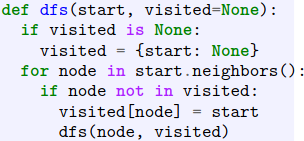
\includegraphics[scale=0.25]{dfs.png}\\
discovery edges: the edges that we take to discover a new node\\
non-tree edges: other edges\\
back edges: the edges to an ancestor in the DFS tree\\
forward edges: the edges to a descendant node in the DFS tree\\
cross edges: the edges to a non-ancestor/non-descendant node\\
properties: discovery edges form a spanning tree of the connected component; if a node v is connected to the start node, there is a path from the start node to v in the DFS tree; visits each node and check each edge once (twice for undirected graphs); complexity is O(n+m) for n nodes and m edges
}\\
\scriptsize{BFS}\\ {\tiny explore all options in parallel, divides the nodes into level (starting node at level 0...)\\
typically implemented with a queue\\
if replace the queue with a stack, it is an iterative version of DFS\\
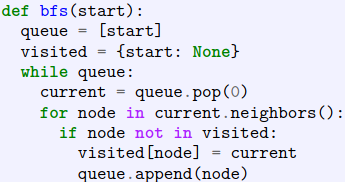
\includegraphics[scale=0.25]{bfs.png}\\
shortest path: if a node v is reachable from the start node, BFS finds the shortest path from the start node to v\\
complexity: O(n+m)
}\\
\scriptsize{find path}\\ {\tiny traverse the graph from the source code, record the discovery edges\\
start from the target node, trace the path back to the source\\
with BFS, we get the shortest path\\
running time is the length of the path O(n)\\
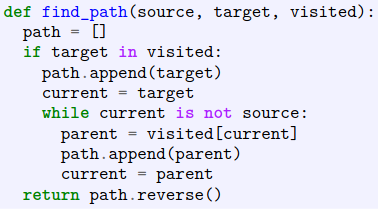
\includegraphics[scale=0.25]{find-path.png}
}\\
\scriptsize{test connectivity, find connected components, find cycle}\\
{\tiny connected: yes if the "visited" nodes have the same length as the graph nodes\\
find the connected components: run traversal multiple times until all nodes are visited\\
cyclic: yes if there is a back edge during graph traversal
}
\subsection*{Directed graphs}
\scriptsize{terminology}\\
{\tiny for any pair of nodes u and v, a directed graph is\\
strongly connected: if there is a directed path between u to v and v to u\\
semi-connected: if there is a directed path between u to v or v to u\\
weakly connected: if the undirected graph obtained by replacing all edges with undirected edges is a connected graph
}\\
\scriptsize{check strong connectivity}\\
{\tiny naive attempt: traverse the graph independently from each node (strongly connected if all traversals visit all nodes)\\
time complexity O(n(n+m))\\
better:\\ 
1. traverse the graph from an arbitrary node\\
2. reverse all edges, traverse again\\
3. intuition: if there a reverse path from D to A, then D is reachable from A\\
time complexity: O(n+m)
}\\
\scriptsize{transitive closure} {\tiny another graph where:\\
-the set of nodes are the same as the original graph\\
-there is an edge between two nodes u and v if v is reachable from u\\
for undirected graph, can be computed by computing the connected components\\
a straightforward algorithm:\\
1. run n graph traversals from each node in the graph\\
2. add an edge between the start node to any node discovered by the traversal\\
time complexity O(n(n+m))\\
(note: in a dense graph m is O(n**2))\\
Floyd-Warshall algorithm: efficient if graph is implemented with an adjacency matrix and is not sparse\\
1. setting transitive closure to the original graph\\
2. for k=1...n, add a directed edge (vi,vj) to transitive closure if it already contains both (vi,vk) and (vk,vj)\\
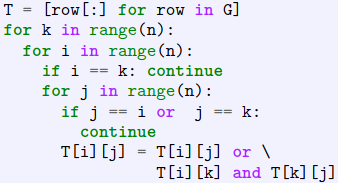
\includegraphics[scale=0.25]{floyd-warshall.png}\\
time complexity O(n**3)\\
a version of this is used for finding shortest paths in weighted graphs
}\\
\scriptsize{Directed acyclic graphs(DAGs)} {\tiny directed graphs without cycles\\
applications: course dependence, class inheritance, scheduling constrains over tasks in a project, dependency parser output\\
topological order: a sequence of nodes such that for every directed edge (u,v) u is listed before v; there may be multiple topological orderings, e.g. any acceptable order that the courses can be taken\\
topological sort:\\
1. keep record of number of incoming edges\\
2. a node is ready to be placed in the sorted list if there are no unprocessed incoming edges\\
time complexity O(n+m)\\
if topological ordering does not contain all the edges, the graph includes a cycle\\
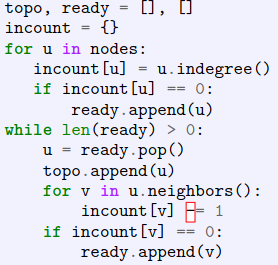
\includegraphics[scale=0.25]{topo-sort.png}
}
\subsection*{Shortest Paths}
\scriptsize{weighted graph}
{\tiny weights can be any numeric value, but some algorithms require non-negative weights or Euclidean weights (weights that are proper distance metrics)\\
weights often indicate distance or cost, but can also represent positive relations (e.g. affinity between nodes)\\
weight of a path: the sum of weights of the edges on the path
}\\
\scriptsize{shorted paths}\\
{\tiny applications: navigation, routing in computer networks, optimal construction of electronic circuits, robotics, transportation, finance...\\
shortest path on unweighted graphs: a BFS search tree\\
shortest path on unweighted graphs: different versions of the problem, restrictions on weights
}\\
\scriptsize{Dijkstra's algorithm} {\tiny a weighted version of BFS, finds shorted path from a single source node to all connected nodes\\
weights have to be non-negative\\
a greedy algorithm, grows a 'cloud' of nodes for which we know the shortest paths from the source node\\
new nodes are included in the cloud in order of their shortest paths from the source node\\
1. maintain a list D of minimum known distances to each node\\
2. at each step:\\
-take closest node out of Q\\
-update the distances of all nodes\\
3. can be more efficient if Q is implemented using a priority queue\\
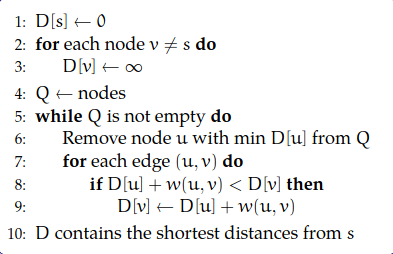
\includegraphics[scale=0.2]{Dijkstra_algo.png}
\\
complexity: in general $O(t_{find-min}n+t_{update-key}m)$\\
with list-based implementation of Q: O(m+n**2)=O(n**2)\\
with a priority queue: O((m+n)logn)\\
similar to traversal algorithms, does not give the shortest-path tree, but can be extracted from distances D, running time O(n**2) or O(n+m)\\
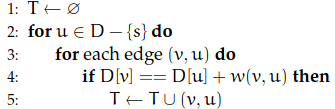
\includegraphics[scale=0.2]{path_tree.png}
\\
}
\scriptsize{Shortest paths on DAGs}
{\tiny directed acyclic graphs\\
similar to Dijkstra's, but simpler and faster\\ 
only difference is to follow a topological order\\
will also work with negative edge weights
}\\
\scriptsize{Bellman-Ford algorithm}
{\tiny single-source shortest path problem for directed graph\\
include cycles, negative weights, exclude negative cycles\\ 
1. similar to earlier algorithms, initialize D[s]=0, D[v]=infinity\\
2. make n passes over the edges:\\
-update distances for each edge (relax edges)\\
-stop if there were no changes at the end of a pass
}
\subsection*{Minimum Spanning Tree}
\scriptsize{spanning tree}\\
{\tiny - spanning graph: includes all nodes\\
tree - acyclic, connected
}\\
\scriptsize{minimum spanning tree}\\
{\tiny applications: network design, cluster analysis, traveling salesman problem, object/network recognition in images, avoidig cycles in broadcasting, dithering in images audio video, error correction codes, dna sequencing
}\\
\scriptsize{'cut property'}\\ {\tiny a cut of a graph is a partition that divides its nodes into two disjoint (non-empty) sets\\
given any cut, the edge with the lowest weight across the cut is in the MST
}\\
\scriptsize{Prim-Jarnik algorithm} {\tiny
greedy algorithm, finding MST for weighted undirected graph\\
1. starts with a single 'start' node, grows the MST greedily\\
2. at each step:\\
-consider a cut between nodes visited and the rest of the nodes\\
-select the minimum edge across the cut\\
3. repeat the process until all nodes are visited\\
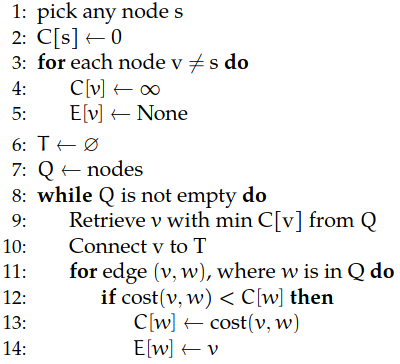
\includegraphics[scale=0.2]{prim-jarnik.png}
\\
complexity: two loops over number of nodes, O(n**2) if we need to search\\
if use a priority queue for Q, O(mlogm)\\
with a priority queue: O((m+n)logn)
}\\
\scriptsize{Kruskal's algorithm}
{\tiny finding MST on undirected graphs\\
1. start with each node in its own partition\\ 
2. at each iteration, choose the edge with the minimum weight across any two clusters, and join them\\
3. terminates when there are no clusters to join\\
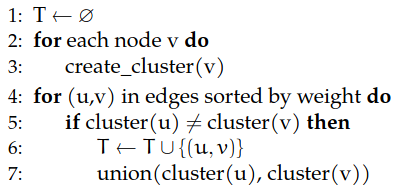
\includegraphics[scale=0.2]{kruskals_algo.png}
\\
loop over edges, but beware of the sorting requirement\\
O(mlogm) with simple data strcutures
}\\
\scriptsize{Directed trees}\\
{\tiny -rooted directed tree (arborescence): an acyclic directed graph where all nodes are reachable from the root node through a single directed path (what computational linguists simply calls a tree)\\
- anti-arborescence: a rooted directed tree where all edges are reversed\\ 
- polytree (a drected tree): a directed graph where undirected edges form a tree\\
finding an MST in a directed graph = finding a rooted directed tree
}\\
\scriptsize{Chu-Liu/Edmonds algorithm}\\
{\tiny 1. the MST for a directed graph has to start from a designated root node\\
- if selected node has any incoming edges, remove them\\ 
- common practice to introduce an artificial root node with equal-weight edges to all ndoes\\
2. for all non-root nodes, select the incoming edge with lowest weight, remove others\\
3. if the resulting graph has no cycles, it is an MST
4. if there are cycles, break them\\
- consider the cycle as a single node
- select the incoming edge that yields the lowest cost if used for breaking the cycle
5. repeat until no cycles remain\\
generally defined recursively: at each step, create a new graph with a contracted cycle call the procedure with the new graph\\
at most n recursions: the cycle has to include more nodes at every step\\
at each call, m steps for finding minimum incoming edge (also finding a cycle with O(n), but m>=n)\\
the vanilla algorithm runs in O(mn), there are improved versions\\
in CL dependency parsing:\\
1. begin with fully connected weighted graph, except the root node has no incoming edges\\
2. weights are estimated from a treebank, typically determined by a machine learning method trained on a treebank\\
3. often use probabilities, i.e. maximize the weight of the tree\\
4. one of the most common (and successful) approaches to dependency parsing
}
\section{Maps \& Hash Tables}
\scriptsize{hash function}\\ 
{\tiny a one-way function that takes a variable-length object and turns it into a fixed-length bit string\\
most common application: set, map (associative array/dictionary/symbol table)\\
other applic.: database indexing, cache management, efficient duplicate detection, file signature verification against corrupt/tempered files, password storage, electronic signatures, part of many cryptographic algorithms/applications
}\\
\scriptsize{set}\\ {\tiny abstract data type, unordered collection without duplicates\\
basic operations: x in s, s.add(x), s.remove(x)
}\\
\scriptsize{map}\\ {\tiny abstract data type, a collection that allows indexing with almost any data type (Python dict require immutable data type)\\
basic operations: d[key], d[key]=val, del d[key]
}\\
{\tiny implement sets and maps:\\}
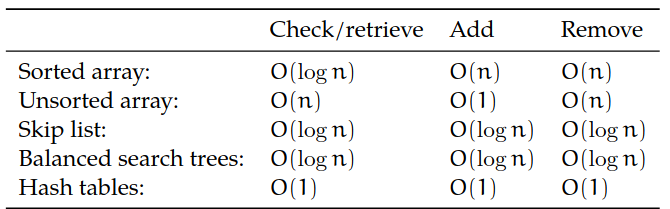
\includegraphics[scale=0.15]{sets_maps.png}\\
\scriptsize{hash function}\\
{\tiny h() maps a key to an integer index between 0 and m(size of array)\\
we use h(k) as an index to an array(of size m)\\
collision: occurs if 2 different key values are mapped to the same integer\\
2 parts: map any object (variable bit string) to an integer (e.g., 32 or 64 bit); compress the range of integers to map size(m)\\
main challenge with implementing hash maps: avoid and handle the collisions
}\\
\scriptsize{compress hash codes}\\ 
{\tiny easy way: use modulo m+1 to map any integer to range [0,m]\\
good hash functions minimize collisions, but collisions occur\\
2 common approaches to handle collisions: separate chaining, open addressing
}\\
\scriptsize{separate chaining} {\tiny each array element keeps a pointer to a secondary container(typically a list); when an collision occurs, add the item to the list\\
complexity: all operations require locating the element first, cost include hashing(constant)+search in secondary data structure, worst-case O(n)\\
with a good hash function, the probability of collision is n/m, O(n/m)=O(1) (if m>n)\\
expected complexity for all operations is O(1)
}\\
\scriptsize{load factor} {\tiny = num of entries/num of indices\\
low load factor: better run time (fewer collisions)/more memory usage\\
when load factor is over a threshold, the map is extended(needs rehash)\\
around 0.75 is considered optimal
}\\
\scriptsize{open addressing(linear probing)} {\tiny during insertion, if there is a collision, look for the next empty slot and insert\\
during lookup, probe until there is an empty slot\\
when delete an element, insert a special value that is treated as full during lookup and empty during insertion\\
tends to create clusters of items, especially if load factor is high(>0.5)\\
quadratic probing provides some improvement
}\\
\scriptsize{quadratic probing} {\tiny prob (h(k)+i**2) mod m for i=0,1,... until an empty slot is found\\
if m is prime and load factor is less than 0.5, guaranteed to find an empty slot\\
although better than linear probing, creates its own kind of clustering
}\\
\scriptsize{double hashing} {\tiny prob (h(k)+i*h'(k)) mod m for i=0,1,..., where h'(k) is another hash function\\
common choice: h'(k)=q-(k mod q) for a prime number q<m
}\\
\scriptsize{pseudo random number generator}
{\tiny prob $(h(k)+i*r_i) mod m$ for i=0,1,..., where $r_i$ is the i-th number generated by a peudo number generator\\
pseudo random number generators generate numbers that are close to uniform, given the same seed, the sequence is deterministic\\
the most common choice for modern programming languages, avoids problems with inputs that intentionally generate hash collisions
}\\
\scriptsize{has DoS attachs}\\ {\tiny a denial-of-service(DoS) attach aims to break or slow down an internet site/service\\
input to a web-based program is passed as key-value pairs, which are typically stored in a dictionary\\
if one intentionally posts an input with large number of colliding keys, the hash table implementation needs to chain long sequences or probe large number of times and eventually re-hash\\
this increases expected to O(1) time to worst-case complexity
}\\
\scriptsize{xor or add}\\
{\tiny hash codes must be consistent: if a==b, h(a)==h(b)\\
should minimize collisions, values for h should be uniformly distributed\\
should be fast to compute (or not if used for passwords\\
simple appraoch: bitwise add (or XOR) each k-bit segment of the memory representation of the object, ignoring the overflow\\
in practice create many collisions due to associativity (abc, bca and cba get the same hash code)
}\\
\scriptsize{polynomial hash codes}\\
{\tiny multiply with powers of a constant, will produce different values with sequences with the same items in different order\\
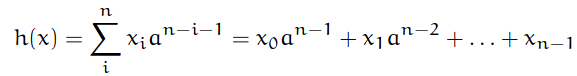
\includegraphics[scale=0.2]{poly_hash.png}
}\\
\scriptsize{cyclic-shift hash codes}\\
{\tiny shifts some bits from one end to the other at each step in the running sum\\
a fast way of obtaining a non-associative valid hash code since bitwise operations are simple \\
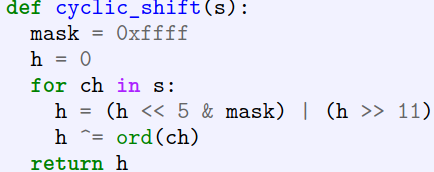
\includegraphics[scale=0.2]{cyclic_shift.png}
}\\
\scriptsize{cryptographic hash functions} {\tiny in cryptography, it is important to have hash functions for which it is difficult to find two keys with the same hash value\\
well-known hash functions: MD5, SHA-1, RIPEMD-160, Whirlpool, SHA-2, SHA-3, BLACK2, BLACK3\\
designed for applications like digital fingerprinting, password storage\\
computationally inefficient for use in data structures
}
\section{String Matching}
{\tiny find all occurrences of pattern p (length m) in text t (length n) \\
The size of the alphabet (q) is often an important factor\\
p occurs in t with shift s if p[0:m] == t[s:s+m]\\
A string x is a prefix/suffix of string y, if y=xw/ y=wx for a possibly empty string w\\}\\
\scriptsize{Brute-force string search}\\ 
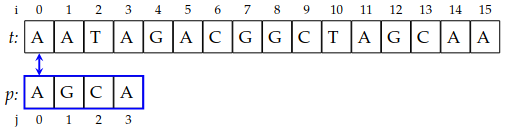
\includegraphics[scale=0.25]{string-match.png}\\{\tiny Start from the beginning, of i = 0 and j = 0\\
-if j == m, announce success with s = i\\
-if t[i]! = p[j]: shift p (increase i, set j = 0)\\
-otherwise: compare the next character (increase i and j, repeat)\\
worst case: t: AAAAAAAAC, p: AAC}\\
\scriptsize{Boyer-Moore algorithm}\\
{\tiny start comparing from the end of p\\
If t[i] does not occur in p, shift m steps\\
Otherwise, align the last occurrence of t[i] in p with t[i]\\
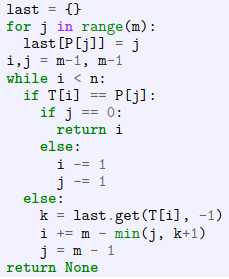
\includegraphics[scale=0.25]{boyer-moore.png}\\
on average performs better than brute-force\\
wost case complexity O(nm), e.g. t=aaaaaaa, p=baa\\
faster version exists O(n+m+q)
}\\
\scriptsize{FSA}\\
{\tiny 1. start at state 0, switch states based on the input\\
2. all unspecified transitions go to state 0\\
3. when at the accepting state, announce success\\
naive attemp building automaton O(qm**3)\\
matching O(n)\\
space requirement O(qm) if stored in matrix\\
faster algorithms for construction exists
}\\
\scriptsize{Knuth-Morris-Pratt (KMP) algorithm}\\ {\tiny 1. in case of a match, increment both i and j\\
2. on failure, or at the end of the pattern, decide which new p[j] compare with t[i] based on a function f\\
3. f[j-1] tells which j value to resume the comparisons from\\
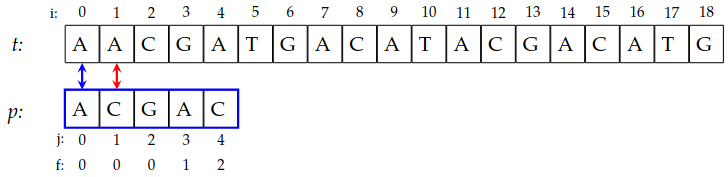
\includegraphics[scale=0.25]{kmp-demo.png}\\
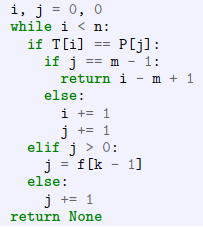
\includegraphics[scale=0.25]{kmp.png}\\
either increase i or shift the comparison\\
runs at most 2n times, complexity O(n)\\
build prefix/failure table\\
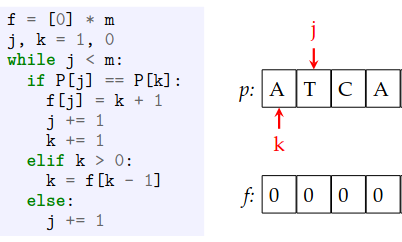
\includegraphics[scale=0.25]{failure-table.png}
}\\
\scriptsize{Robin-Karp algorithm}\\ {\tiny 1. instead of matching the string itself, matching the hash of it (based on a hash function)\\
2. If a match found, we need to verify – the match may be because of a hash collision\\
3. Otherwise, the algorithm makes a single comparison for each position in the text\\
a hash should be computed for each position (size m) (rolling hash functions avoid this complication)
}\\
\scriptsize{rolling hash function} {\tiny changes the hash value only based on the item coming in and going out of the window\\
to reduce collisions, better rolling-hash functions (e.g. polynomial hash functions) can be used
}
\section{String Edit Distance}
{\tiny typically formulated as the (inverse) cost of obtaining one of the strings from the other through a number of edit operations \\
once we obtain the optimal edit operations, we may also be able to determine the optimal alignment between the strings}\\
\scriptsize{Hamming distance}\\ 
{\tiny number of different symbols in the corresponding positions\\
easy calculation, but cannot handle sequences of different lengths}\\
\scriptsize{Longest common subsequence (LCS)}\\
{\tiny an order-preserving sequence of symbols from a string (solved by UNIX diff)\\
e.g. LCS(hygiene, hygeine) = hygine / hygene\\
naive solution:\\
1. Enumerate all subsequences of the first string (exponential)\\
2. Check if it is also a subsequence of the second string\\
O(m2**n) for strings of size n and m\\
recursive definition:\\
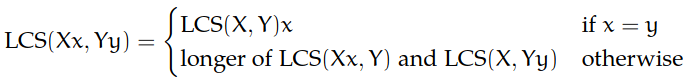
\includegraphics[scale=0.2]{lcs-recursive.png}\\
divide and conquer:\\
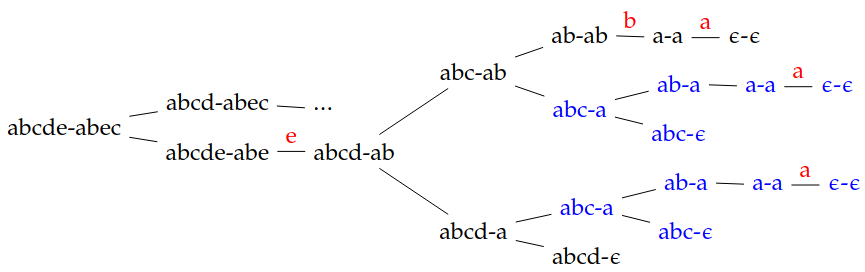
\includegraphics[scale=0.2]{lcs-divide.png}\\
dynamic programming: \\
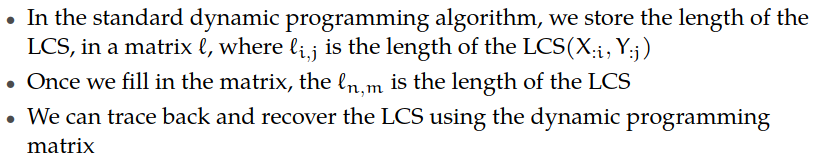
\includegraphics[scale=0.2]{lcs-dynamic.png}\\
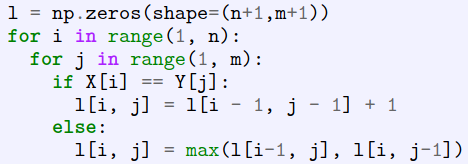
\includegraphics[scale=0.25]{lcs-algo.png}\\
time complexity O(nm), space complexity O(nm)\\
back errors give a set of edit operations (assume original string is the vertical one):\\
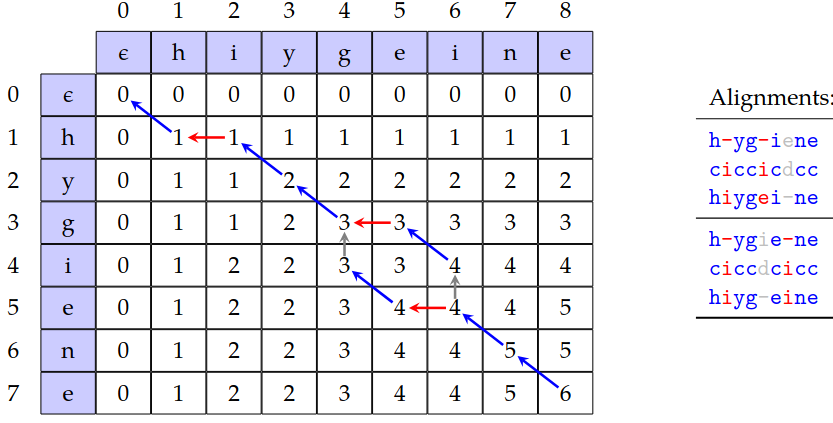
\includegraphics[scale=0.15]{lcs-recover.png}\\
- copy (diagonal arrows in the demonstration)\\
- insert (left arrows in the demo)\\
- delete (up arrows in the demo)\\
cost: copy 0, delete 1, insert 1
}\\
\scriptsize{Levenshtein distance}\\
{\tiny the total cost of insertions, deletions and substitutions\\
naive recursion as in lcs with cost 1 for all operations\\
\texttt{d[i,j]= min(d[i-1,j]+1, d[i,j-1]+1, d[i-1,j-1])}\\
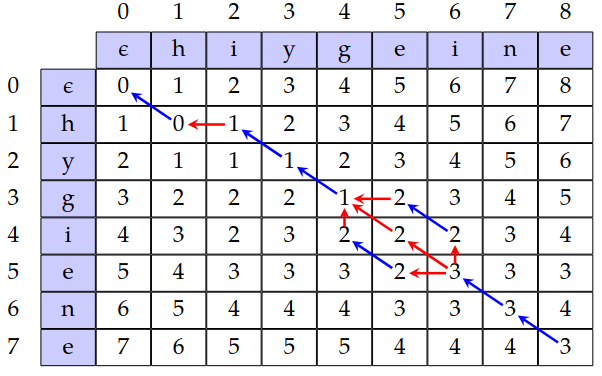
\includegraphics[scale=0.2]{levenshtein.png}
}\\
\scriptsize{swap}\\ {\tiny useful for applications like spell checking
}
\section{Tries}
{\tiny a trie (or prefix tree) is a tree-based data structure, particularly used for fast
pattern matching \\
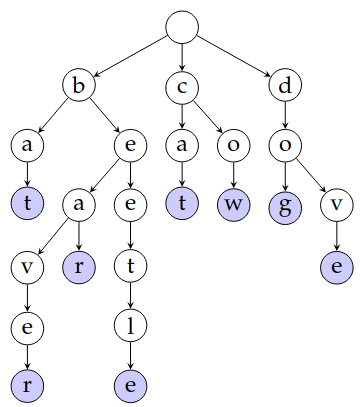
\includegraphics[scale=0.2]{trie.png}\\
}\\
\scriptsize{search}\\ 
{\tiny start from root, jump to node with current character\\
fail: if there is no character to follow/input ends in a non-leaf node\\
accpet if at a leaf node at the end of the input\\
to prevent that no string is a prefix of another: append a special end-of-string symbol/mark the nodes that correspond to ends of strings}\\
\scriptsize{complexity}\\
{\tiny O(n) for search, insert or delete\\
a factor from the alphabet size q, but can be reduced to O(log q) with binary search, or O(1) if a method allowing direct addressing is used
}\\
\scriptsize{properties}\\
{\tiny Internal nodes may have as many children as the number of symbols in the alphabet (in practice much smaller, averge degree of nodes goes down as the depth increase)\\
height of the trie=longest string\\
num of leaves = num of strings\\
worst case num of nodes=total length of all strings
}\\
\scriptsize{compress} {\tiny replace 'redundant' nodes with nodes labeled with substrings, saves space and may speed up operations
}\\
\scriptsize{suffix tries} {\tiny tries that include all suffixes of a string, O(n) for substring search\\
if the search ends in a leaf node, the pattern is a suffix of the string\\
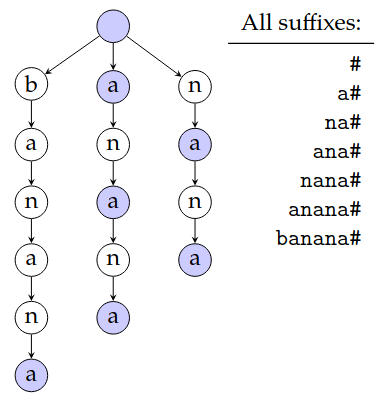
\includegraphics[scale=0.2]{suffix-trie.png}\\
Standard suffix tries use O(n**2) space, compression reduces space requirement to O(n), can be further reduced by keeping indexes to the string rather than the string itself in the (compressed) trie nodes\\
Iterative insertion of suffixes result in a quadratic (O(qn**2)) construction time complexity\\
there are linear time algorithms for constructing suffix tries\\
generalized suffix tries allow storing multiple strings(documents) in a single suffix trie (each string gets a special end-of-string marker)
}\\
\section{Finite State Automata}
{\tiny Every regular language is generated/recognized by an FSA, every FSA generates/recognizes a regular language\\
One of the states is the initial state, some states are accepting states\\
}\\
\scriptsize{Deterministic finite automata(DFA)} 
{\tiny At any state and for any input, a DFA has a single well-defined action to take\\
we can add a sink(or error) state to make all transitions well-defined (for brevity skipped)
}\\
\scriptsize{Non-deterministic finite automata(NFA)}\\ {\tiny transition table cells have sets of states\\
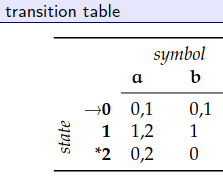
\includegraphics[scale=0.2]{transition-table.png}\\
NFA recognition(with backtracking)\\
1. start at q0\\
2. take the next input, place all possible actions to an agenda (state, character index)\\
3. get the next action from the agenda, act\\
4. at the end of input: accept-if in an accepting state; reject-not in accepting state \& agenda empty; backtrack-otherwise\\
worst time complexity is exponential\\
depth-first search with stack as agenda, breath-first search with queue as agenda\\
machine learning methods to guide a best solution\\
NFA recognition(parallel version)\
1. start at q0\\
2. take the next input, mark all possible next states\\
3. if an accepting state is marked at the end of the input, accept\\
note: the process is deterministic and finite-state\\
}\\
\scriptsize{$\epsilon$-NFA} {\tiny allows moving without consuming an input symbol\\
any $\epsilon$-NFA can be converted to an NFA\\
}\\
\scriptsize{NFA-DFA equivalence}\\
{\tiny the set of DFA is a subset of the set of NFA(DFA is also an NFA)\\
NFA can automatically be converted to the equivalent DFA\\
DFA recognition is O(n), NFA recognition may be exponential\\
NFA are often easier to construct/may require less memory
}\\
\scriptsize{$\epsilon$ removal}\\ 
{\tiny 1. start with finding the $\epsilon$-closure of all states\\
2. replace each arc to each state with arc(s) to all states in the $\epsilon$-closure\\
with transition table:\\
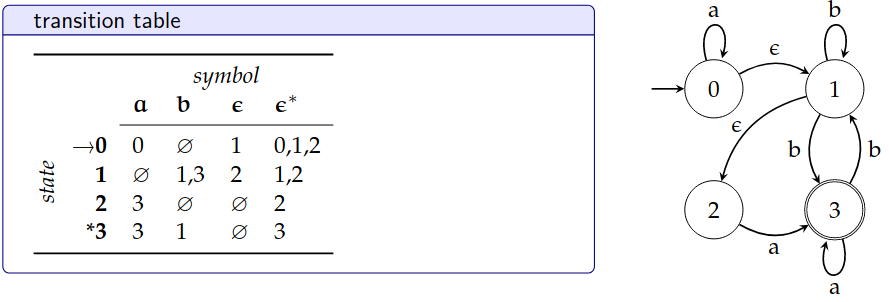
\includegraphics[scale=0.15]{epsilon-removal.png}\\
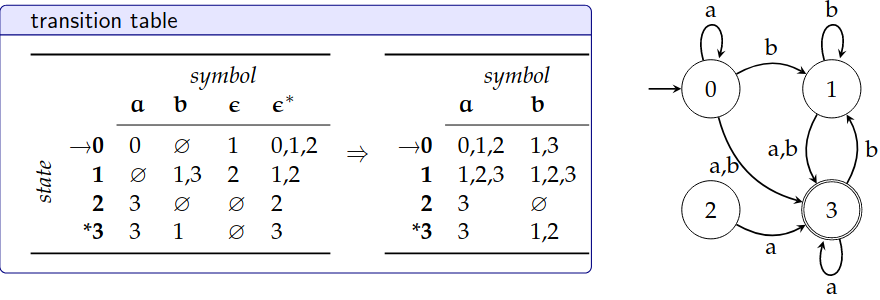
\includegraphics[scale=0.15]{epsilon-removal1.png}
}
\subsection*{NFA Determinization}
\scriptsize{subset construction}\\
{\tiny 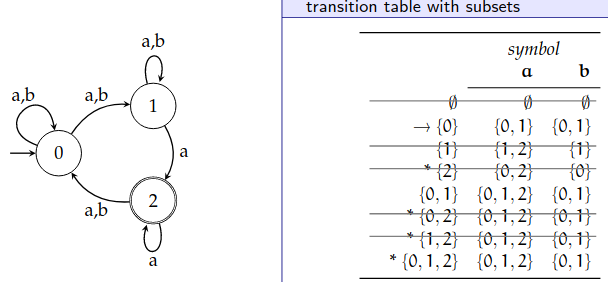
\includegraphics[scale=0.2]{subset-construction.png}\\
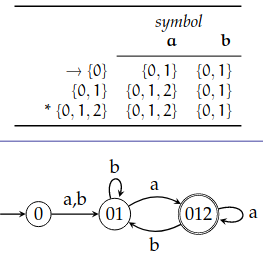
\includegraphics[scale=0.2]{subset-construction1.png}\\
can skip the unreachable states during subset construction
}
\subsection*{FSA Minimization}
{\tiny for any regular language there is a unique minimal DFA\\
throw away unreachable states, merge equivalent states
}\\
\scriptsize{Hopcroft's algorithm}
{\tiny find and eliminate equivalent states by partitioning the set of states\\
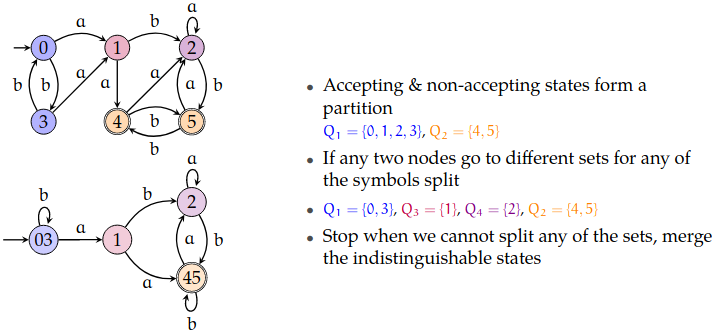
\includegraphics[scale=0.2]{partitioning.png}\\
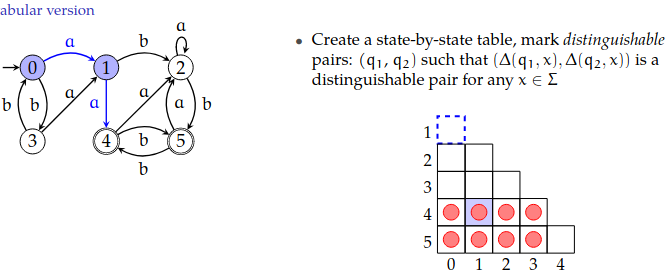
\includegraphics[scale=0.2]{partitioning-tabular.png}\\
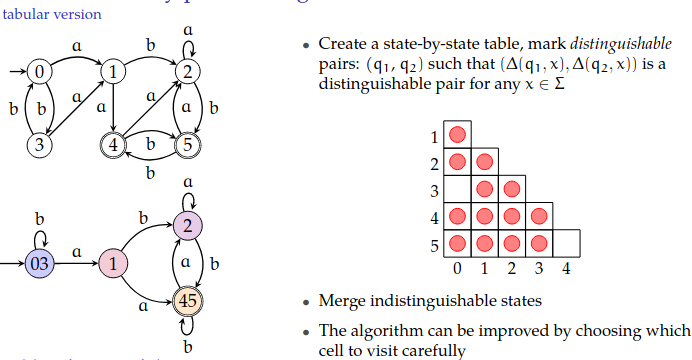
\includegraphics[scale=0.2]{partitioning-tabular1.png}\\
O(n log n) complexity
}\\
\scriptsize{Brzozowski’s algorithm} {\tiny 'double reversal'\\
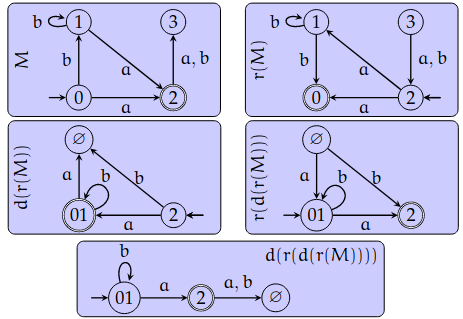
\includegraphics[scale=0.2]{brzozowski.png}\\
exponential worst-time complexity\\
can also be used with NFAs(resulting in the minimal equivalent DFA)
}
\subsection*{Finite State Transducers}
{\tiny The machine moves between the states based on an input symbol, while it outputs the corresponding output symbol\\
The relation defined by an FST is called a regular (or rational) relation\\
we treat an FSA as a simple FST that outputs its input\\
FST share many properties of FSAs, however:\\
- FSTs are not closed under intersection and complement\\
- we can compose(and invert) FSTs\\
- determinizing FSTs is not always possible
}\\
\scriptsize{FST inversion (M**-1)}\\
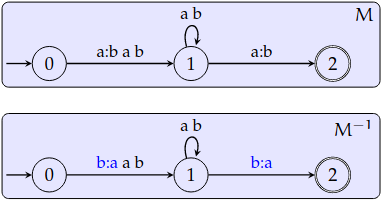
\includegraphics[scale=0.2]{fst-inversion.png}\\
\scriptsize{FST composition}\\ {\tiny sequential application:\\ 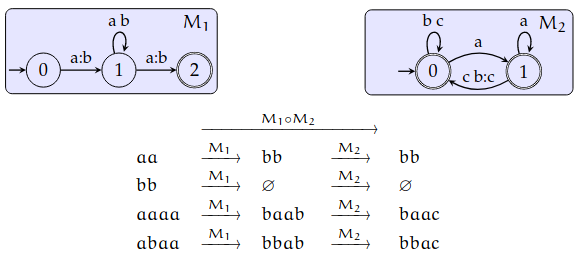
\includegraphics[scale=0.2]{fst-composition.png}\\
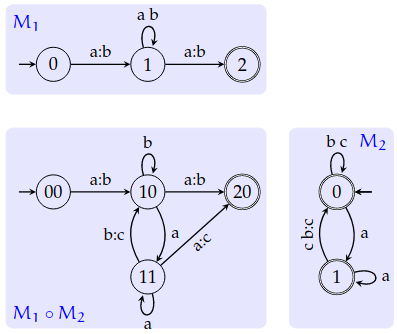
\includegraphics[scale=0.2]{fst-composition1.png}
}\\
\scriptsize{FST projection} {\tiny
turns an FST into a FSA, accepting either the input language or the output language\\
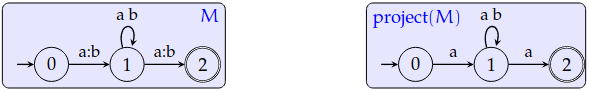
\includegraphics[scale=0.2]{fst-projection.png}
}\\
\scriptsize{FST determinization} {\tiny
means converting to a subsequential FST\\
can extend the subset construction to FSTs\\
not all FSTs can be determinized\\
}\\
\scriptsize{sequential FSTs} {\tiny
has a single transition from each state on every input symbol\\
Output symbols can be strings, as well as $\epsilon$\\
linear recognition time\\
do not allow ambiguity\\
}\\
\scriptsize{subsequential FSTs} {\tiny
A k-subsequential FST is a sequential FST which can output up to k strings at an accepting state\\
allow limited ambiguity\\
linear recognition time\\
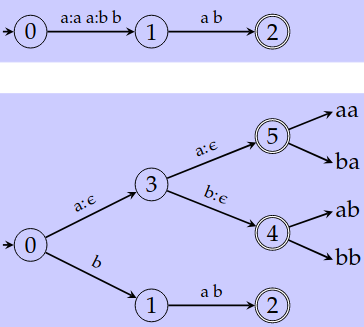
\includegraphics[scale=0.2]{fst-determinization.png}
}\\
\end{multicols*}
\end{document}